\chapter{Конструкторская часть}
\normalsize
Рассмотрим следующие алгоритмы посика для строк для строк $S_1,S_2$  c длиной $L_1, L_2$ соответственно:
\begin{enumerate}
	\item линейный алгоритм поиска расстояния Левенштейна;
	\item рекурсивный алгоритм поиска расстояния Левенштейна;
	\item рекурсивный алгоритм поиска расстояния Левенштейна c кешированием;
	\item линейный алгоритм поиска расстояния Дамерау---Левенштейна.
\end{enumerate}

\section{Линейный алгоритм поиска расстояния Левенштейна}
\label{subsec:levenshteinDistanceSimple}
Этот алгоритм реализуется с использованием матрицы размером $L_1 + 1$ на $L_2 + 1$. Номер строки матрицы $i$ соответствует длине подстроки $S_1$, а номер столбца $j$~---~длине подстроки $S_2$ сответственно. Значение элемента матрицы $M[i][j]$ соответствует расстоянию Левенштейна между подстроками $S_1[1..i]$, $S2[1..j]$. Для вычисления значения элемента $M[i][j]$ используется формула~~(\ref{eq:lev_req}).


\section{Рекурсивный алгоритм поиска расстояния Левенштейна}
\label{subsec:levenshteinDistanceRecurcive}
При использовании рекуррентной формулы возможно использование рекурсии. Функция принимает на вход 2 строки, а также их длины на данный момент. После рассмотрения строк с длинами $i$ и $j$, необходимо рассмотреть те же строки с длинами $(i-1, j-1)$, $(i, j-1)$, $(i-1, j)$ и рассчитать их стоимость с помощью формулы (\ref{eq:lev_req}). Среди всех рассмотренных стоимостей строк необходимо на каждом шаге выбрать вариант с наименьшей стоимостью из возможных.

\section{Рекурсивный алгоритм поиска расстояния Левенштейна c кешированием}
\label{subec:levenshteinDistanceRecurciveCache}
При реализации предыдущего рассмотренного метода можно запоминать уже посчитанные значения, чтобы использовать их в дальнейшем и не пересчитывать заново. Кеширование реализуется с использованием матрицы, аналогичной той, которая использовалась в пукте \ref{subsec:levenshteinDistanceSimple}. Все ячейки этой матрицы изначально заполняются значением $+\infty$. Перед вычислением текущего значения происходит проверка: в случае, если значение $M[i][j] = +\infty$, вычисляется текущее значение и заносится в матрицу, иначе
вычисления значения не происходит и оно берется из ячейки $M[i][j]$.

\section{Линейный алгоритм поиска расстояния Дамерау---Левенштейна}
\label{subec:damerauLevenshteinDistanceSimple}
Этот алгоритм реализуется с использованием матрицы размером $L_1 + 1$ на $L_2 + 1$. Номер строки матрицы $i$ соответствует длине подстроки $S_1$, а номер столбца $j$~---~длине подстроки $S_2$ сответственно. Значение элемента матрицы $M[i][j]$ соответствует расстоянию Левенштейна между подстроками $S_1[1..i]$, $S2[1..j]$. Для вычисления значения элемента $M[i][j]$ используется формула~~(\ref{eq:dam_lev_req}).

\section{Схемы алгоритмов}
\begin{figure}[H]
	\centering
	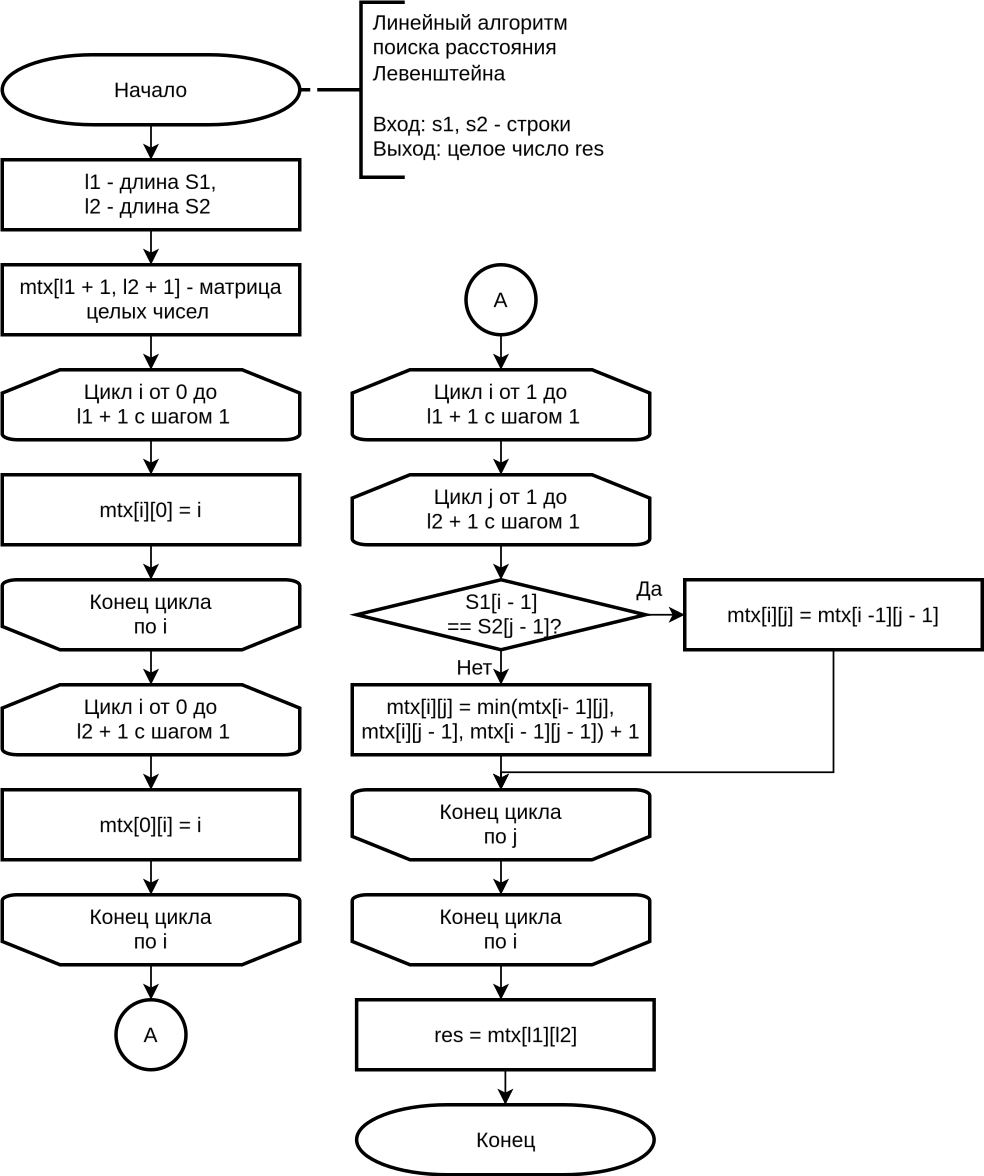
\includegraphics[width=1\textwidth]{inc/img/lev_alg.pdf}
	\caption{Схема линейного алгоритма поиска расстояния Левенштейна}
	\label{fig:levenshteinDistanceSimple}
\end{figure}

\begin{figure}[H]
	\centering
	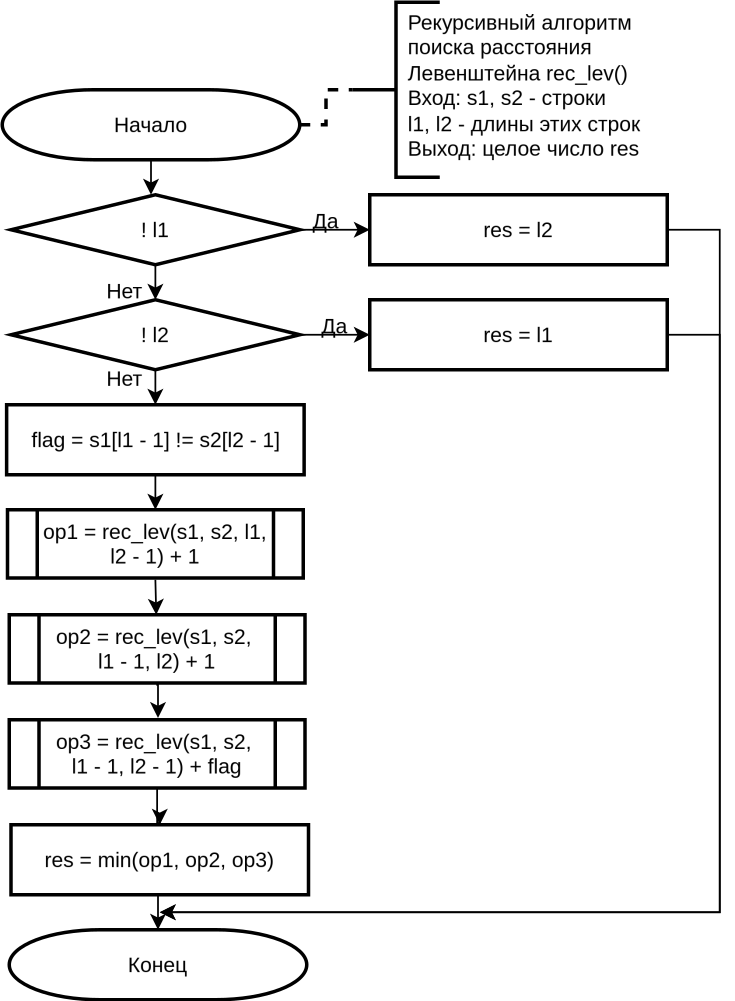
\includegraphics[width=1\textwidth]{inc/img/rec_lev_alg.pdf}
	\caption{Схема реккурсивного алгоритма поиска расстояния Левенштейна}
	\label{fig:levenshteinDistanceRecurcive}
\end{figure}

\begin{figure}[H]
	\centering
	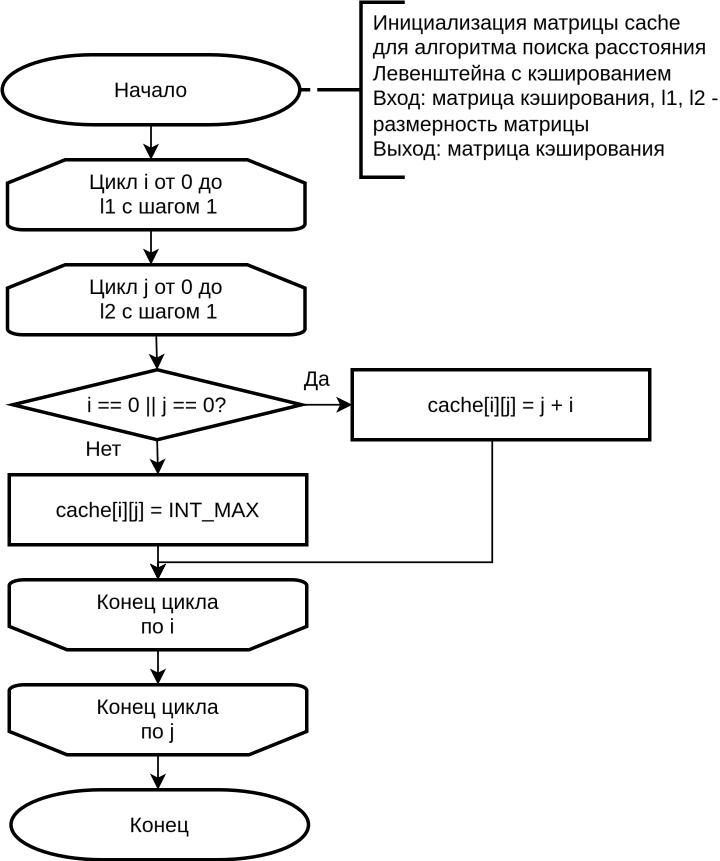
\includegraphics[width=1\textwidth]{inc/img/cahce_prep.pdf}
	\caption{Инициализация матрицы cache для алгоритма поиска расстояния Левенштейна с кешированием}
	\label{fig:levenshteinDistanceRecurciveCachePrep}
\end{figure}

\begin{figure}[H]
	\centering
	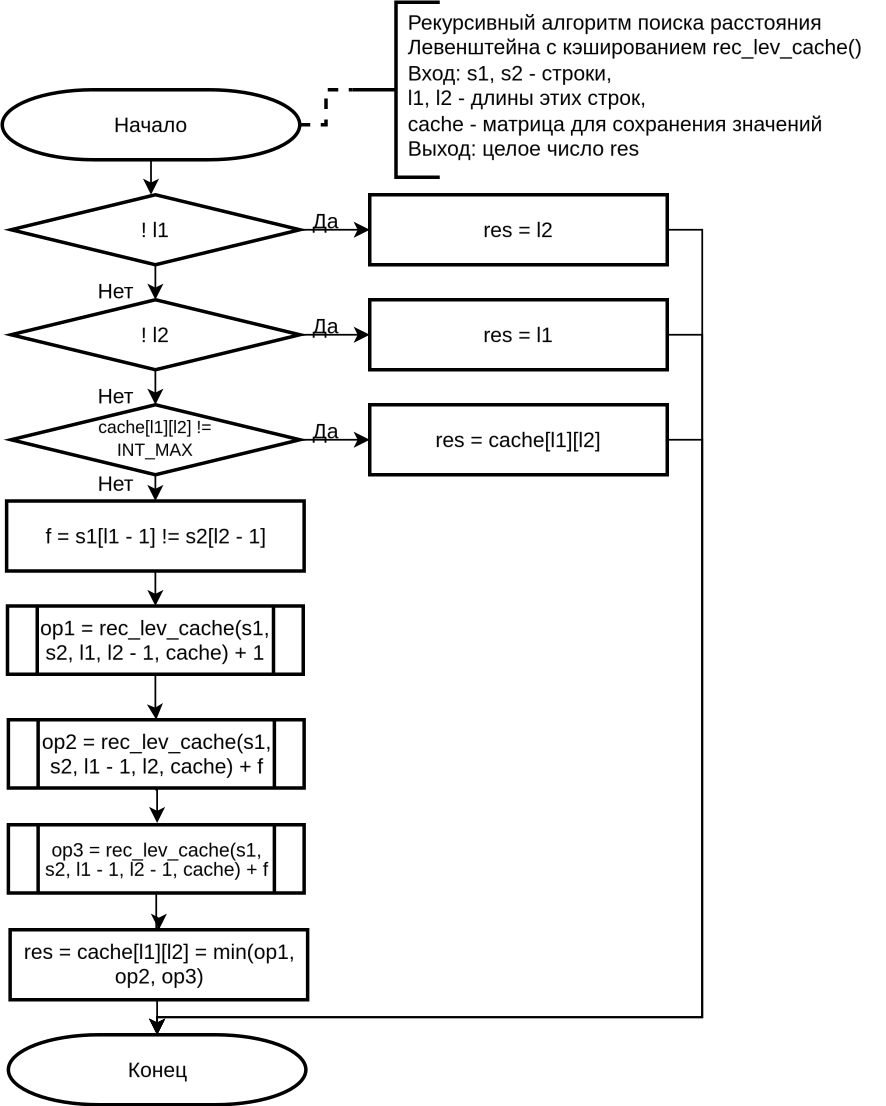
\includegraphics[width=1\textwidth]{inc/img/rec_lev_cache.pdf}
	\caption{Схема реккурсивного алгоритма поиска расстояния Левенштейна с кешированием}
	\label{fig:levenshteinDistanceRecurciveCache}
\end{figure}

\begin{figure}[H]
	\centering
	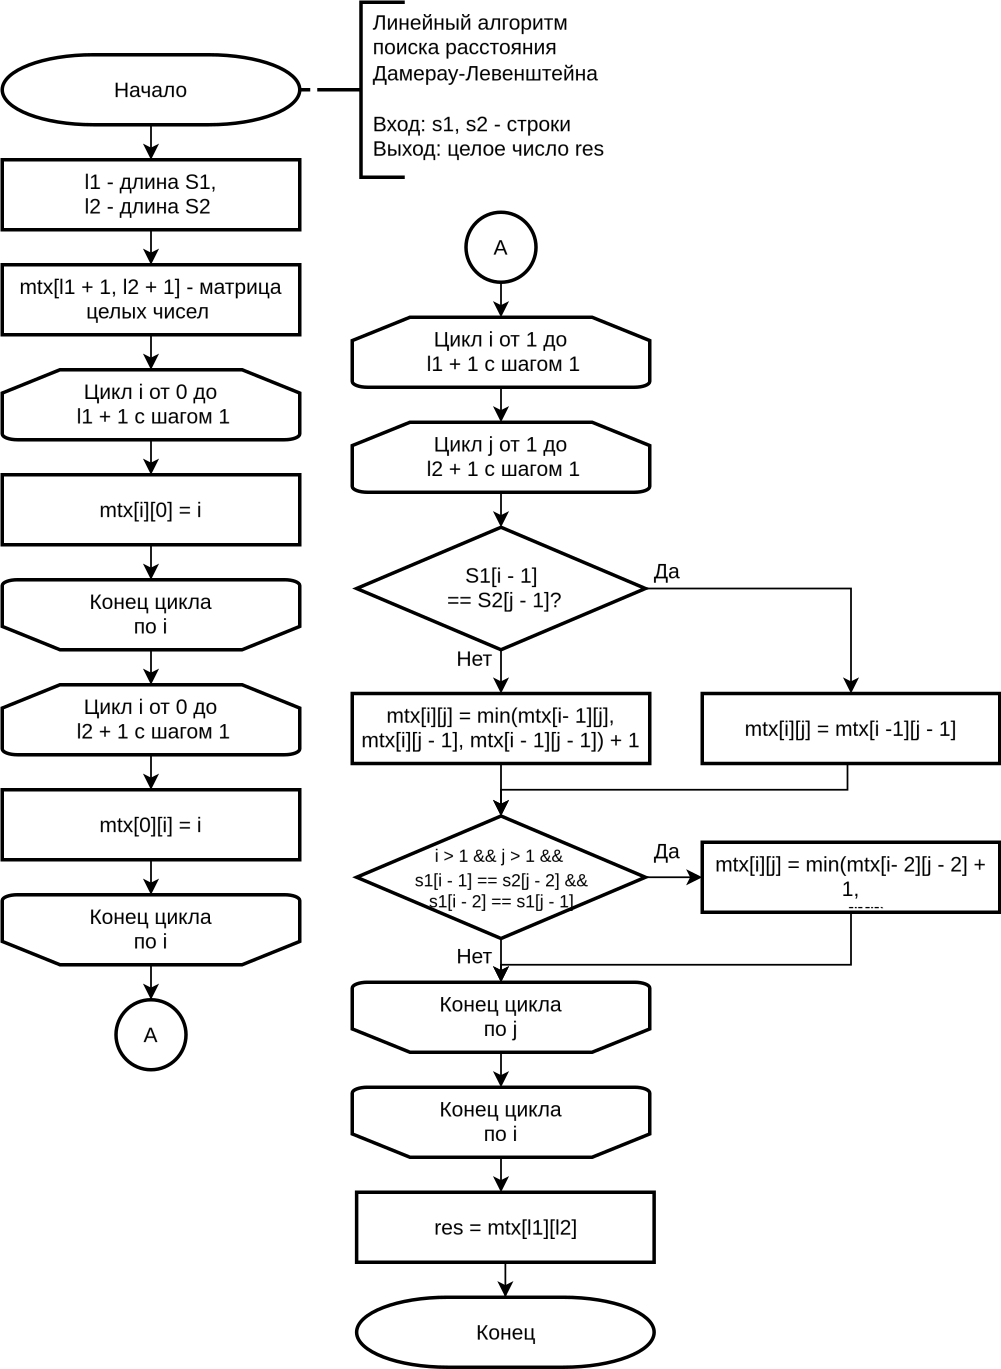
\includegraphics[width=1\textwidth]{inc/img/dam_lev_alg.pdf}
	\caption{Схема линейного алгоритма поиска расстояния Дамерау---Левенштейна}
	\label{fig:damerauLevenshteinDistanceSimple}
\end{figure}
